\documentclass[]{article}

\usepackage{algorithm}
\usepackage{algorithmic}
\usepackage{amsmath}
\usepackage{amssymb}
\usepackage{amsthm}
\usepackage[ngerman,english]{babel}
\usepackage{centernot} 
\usepackage{color}
\usepackage{dsfont}
\usepackage{graphicx}
\usepackage[utf8]{inputenc}
\usepackage{import}
\usepackage{standalone}
\usepackage{qtree}

\usepackage{hyperref}

\title{SOP Challenge - Presentation}
\author{TBD}

\newcommand{\N}{\ensuremath{\mathds{N}}}
\newcommand{\R}{\ensuremath{\mathds{R}}}
\newcommand{\red}[1]{\textcolor{red}{#1}}

\setlength{\itemsep}{-2pt}


\begin{document}
    \maketitle
    \tableofcontents


    %\import{files/}{example_1.tex}

    \section{Remarks on the Tex file and TODOs}

    \begin{itemize}
    	\item \TODO{DPSO text and results}
  		\item \TODO{write conclusion and comparison}
    \end{itemize}

    \section{SOP Problem}

    The Sequential Ordering Problem (SOP) is an asymmetrical TSP with precedence constraints. 

    Each instance of this problem consists of a directed graph $G=(V, A)$, arc weights $w: A \rightarrow \mathbb{R}$, a set of precedence constraints $C \subset V \times V$ as well as a start vertex $s$ and destination vertex $t$.

    The problem consists in finding a permutation of vertices starting at s, ending at t, which satisfy all precedence constraints and minimize the weighted sum of arcs connecting the vertices in the given order. \cite{libralesso2019tree}

    \begin{figure}[hbt]
    	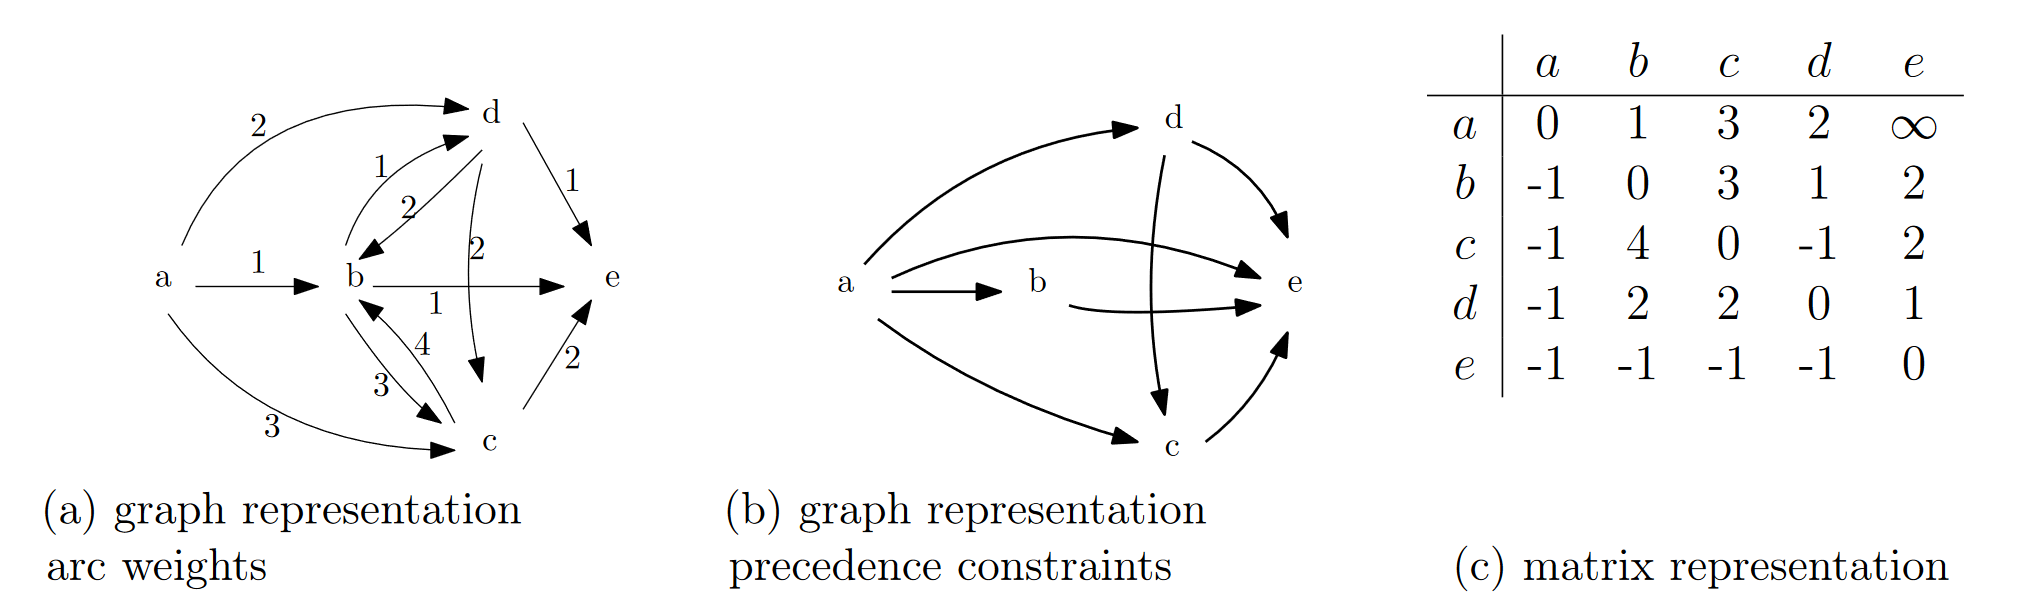
\includegraphics[width=\textwidth]{files/graphic_sop_prob.png}
    	\centering
    	\caption{Illustrative example \cite{libralesso2019tree}}
    \end{figure}



    \section{Solution approaches}

    \subsection{Implemented methods}

    We have implemented multiple methods for solving the SOP Challenge namely an Exact Method and Particle Swarm Optimization Method as well as a Greedy Method and closely related variations of it. In the following we will discuss the latter methods since they have turned out to be the most stable methods in terms finding feasible solutions and computation time in our experiments. We will now give a short description of each of the methods. Tables with results for each of the methods can be found in \ref{results}.

    \subsubsection{Greedy Method}

   	The first, simple heuristic we implemented was a greedy algorithm for the SOP Problem. The Greedy algorithm builds a solution starting from the initial node by choosing the the next best node in terms of cost and precedence constraints. As should be known the greedy algorithm makes local optimal decision which not always lead global optimal solutions. Furthermore the greedy algorithm was able to find feasible solutions for all instances quite fast and is easily implemented due to the local search criteria. \cite{Cormen2009} \\

   	In the case of the SOP Problem the greedy algorithm starts the generation of the Hamiltonian path at the initial node. At each iteration of the algorithm we compute the set of unvisited nodes which do not violate the precedence constraints given by the instance. We then append the node with the lowest cost (greedy selection) for this set to the current path. This procedure repeats until all nodes have been visited and the final node has been reached.

    \subsubsection{GRASP Method}

    \TODO{Add description}

    \subsubsection{Beam Search Method}

    The idea of beam search, in contrast to the greedy algorithm, is to build $K$ different solutions in parallel, where $K$ is called the beam width. For the SOP Problem the algorithms initializes all solution paths from the initial node. It then finds all possible children of the node(s) and computes the cost of each of the new potential paths. To maintain the beam width it selects the $K$ best new paths and repeats these steps until all nodes have been visited and the end vertex has been reached. \cite{Beam:1} \cite{Beam:2} 

    \begin{figure}[hbt]
    	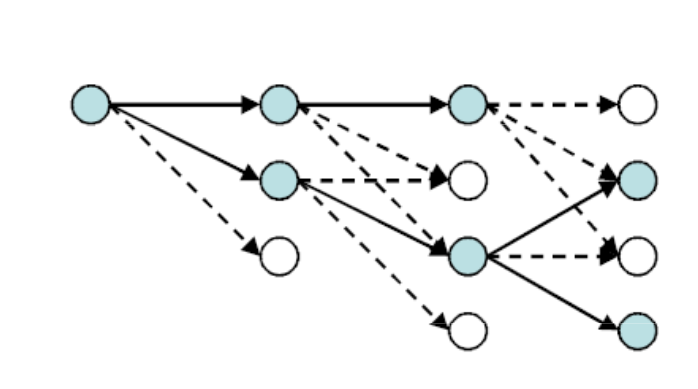
\includegraphics[]{files/beam_search.png}
    	\centering
    	\caption{Beam Search}
    \end{figure}

    \TODO{Add description}

    \subsection{Results}
    \label{results}

    The subsequent tables contain results for the used methods. The first table (\ref{table:results_cost}) displays the costs of the found solutions the second table (\ref{table:results_time}) the time needed to compute the solutions. 

    \begin{table}[htb]
		\rowcolors{2}{gray!25}{white}
		\begin{tabular}{lcccc}
			Instance & LB & UB & Greedy & Beam Search \\
			ESC07 & 2.125 & 2.125 & 2.700 & \\
			ESC11 & 2.075 & 2.075 & 3.175 & \\
			ESC12 & 1.675 & 1.675 & 2.034 & \\
			ESC25 & 1.681 & 1.681 & 3.360 & \\
			ESC47 & 1.288 & 1.288 & 3.843 & \\
			ESC63 & 62	  & 62    & 76 & \\
			ESC78 & 18.230 & 18.230 & 22.600 & \\
			kro124p.1 & 38.762 & 39.420 & 52.575 & \\
			kro124p.2 & 39.841 & 41.336 & 57.723 & \\
			kro124p.3 & 43.904 & 49.499 & 77.266 & \\
			kro124p.4 & 73.021 & 76.103 & 98.427 & \\
			ry48p.1   & 15.805 & 15.805 & 22.493 & \\
			ry48p.2   & 16.074 & 16.666 & 20.911 & \\
			ry48p.3   & 19.490 & 19.894 & 27.342 & \\
			ry48p.4   & 31.446 & 31.446 & 41.176 & \\
			R.500.1000.1  & 1.316   & 1.316 & 6.205 & \\
			R.500.1000.15 & 43.134  & 49.504 & 111.129 & \\
			R.500.1000.30 & 98.987  & 98.987 & 155.387 & \\
			R.500.1000.60 & 178.212 & 178.212 & 205.604 & \\
			R.600.1000.1  & 1.337   & 1.337 & 4.931 & \\
			R.600.1000.15 & 47.042  & 55.213 & 120.975 & \\
			R.600.1000.30 & 126.789 & 126.789 & 189.988 & \\
			R.600.1000.60 & 214.608 & 214.608 & 256.253 & \\
			R.700.1000.1  & 1.231   & 1.231 & 4.886 & \\
			R.700.1000.15 & 54.351  & 65.305 & 151.331 & \\
			R.700.1000.30 & 134.474 & 134.474 & 208.460 & \\
			R.700.1000.60 & 245.589 & 245.589 & 277.504 & \\
		\end{tabular}
		\caption{Results - Cost}
		\label{table:results_cost}
	\end{table}

	\TODO{add some descriptive text}

	\begin{table}[htb]
		\rowcolors{2}{gray!25}{white}
		\begin{tabular}{lcc}
			Instance & Greedy (in s) & Beam Search (in s) \\
			ESC07 & 0.000 & \\
			ESC11 & 0.001 & \\
			ESC12 & 0.001 & \\
			ESC25 & 0.004 & \\
			ESC47 & 0.015 & \\
			ESC63 & 0.026 & \\
			ESC78 & 0.036 & \\
			kro124p.1 & 0.062 & \\
			kro124p.2 & 0.080 & \\
			kro124p.3 & 0.077 & \\
			kro124p.4 & 0.076 & \\
			ry48p.1   & 0.016 & \\
			ry48p.2   & 0.020 & \\
			ry48p.3   & 0.018 & \\
			ry48p.4   & 0.015 & \\
			R.500.1000.1  & 2.617 & \\
			R.500.1000.15 & 25.288 & \\
			R.500.1000.30 & 25.989 & \\
			R.500.1000.60 & 26.161 & \\
			R.600.1000.1  & 4.022 & \\
			R.600.1000.15 & 44.231 & \\
			R.600.1000.30 & 43.502 & \\
			R.600.1000.60 & 43.993 & \\
			R.700.1000.1  & 5.865 & \\
			R.700.1000.15 & 68.580 & \\
			R.700.1000.30 & 69.449 & \\
			R.700.1000.60 & 69.626 & \\
		\end{tabular}
		\caption{Results - Computation Time}
		\label{table:results_time}
	\end{table}





	% references
    \newpage

	\bibliography{references} 
	\bibliographystyle{ieeetr}




\end{document}
